\section{Comparisons}\label{sec:comparisons}

The fundamental problem in comparing Sgr A* models to the data is variability.  We do not expect even an ideal numerical evolution of a source model to match the data point for point, because the space of possible realizations of the model is very large.  But we do expect the {\em distribution} of observables to match an accurate model.  For example, we might expect that the observed 86 GHz flux $F_{86}$ is consistent with being drawn from the distribution of 86GHz fluxes from the model.

Since most observables are correlated over some time $\tau \sim $few $\times 100 G M/c^3$, to obtain the mean and variance of the model distribution to accuracy $f$ we would need a simulation of duration $\sim \tau/f^2 \sim 30,000 (\tau/300) (f/0.1)^{-2}$.  This requires between $10^3$ and $10^4$ node-hours on a state of the art cluster node, depending on the desired resolution, duration, and code used.  This is expensive since $\sim 10$ runs are used for each model set, and runs frequently need to be repeated for multiple values of the numerical parameters (e.g. resolution).  Most of the models used here have been run for either $10,000$ or $30,000 \tg$, although a few have been run to $100,000 \tg$.

The constraints are heterogeneous in the sense that some are related to time-averaged non-contemporaneous measurements (e.g. the NIR flux constraint), while others are instantaneous values measured during the EHT observing campaign (e.g. the m-ring fits), so it is impossible at present to use a single technique to estimate $p$ values for all constraints.

In what follows we will look at each constraint independently (i.e. we will ignore correlations) and generate a $p$ value.  We then cut models with $p < 0.01$.

[CG, Michi to write]

%==============================================================================
\subsection{EHT Constraints}

First we compare data and models using the VLBI null location statistic, the pre-image size, and the ring diameter, ring thickness, and ring asymmetry from m-ring fitting.

It turns out that the null location statistic is informative and tends to rule out edge-on models when $R_{high} > 1$.  The pre-image size statistic is simple but not powerful: most of the models are about the right size, and only a very few face-on, low $R_{high}$ models are too large.   The m-ring fitting is highly informative.  Many of our thermal models look like the data, but - for example - edge on MAD models are large values of $R_{high}$ and positive spin are strongly disfavored because they are too asymmetric.

%==============================================================================
\subsubsection{Null Location}

[CK to summarize]

% Statement about consistency between overlapping model sets.

\begin{figure*}[]
  %\centerline{
  %  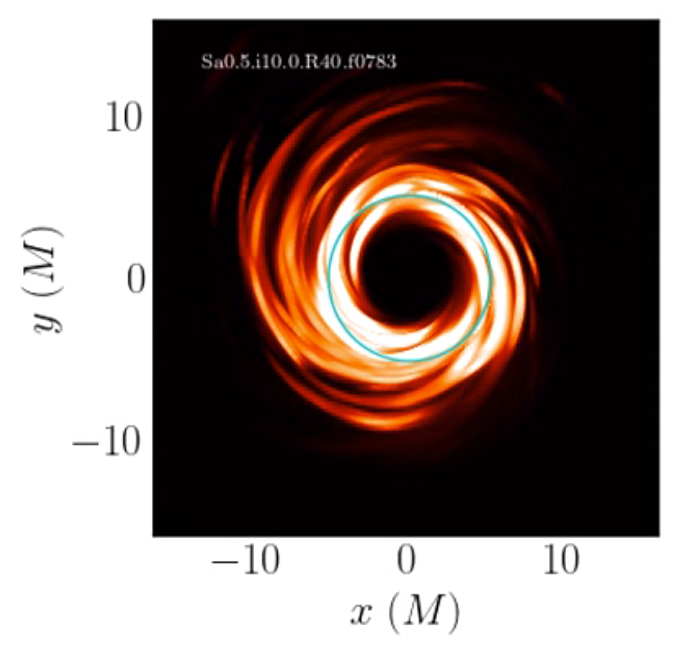
\includegraphics[width=8.5cm]{783_image}%
  %  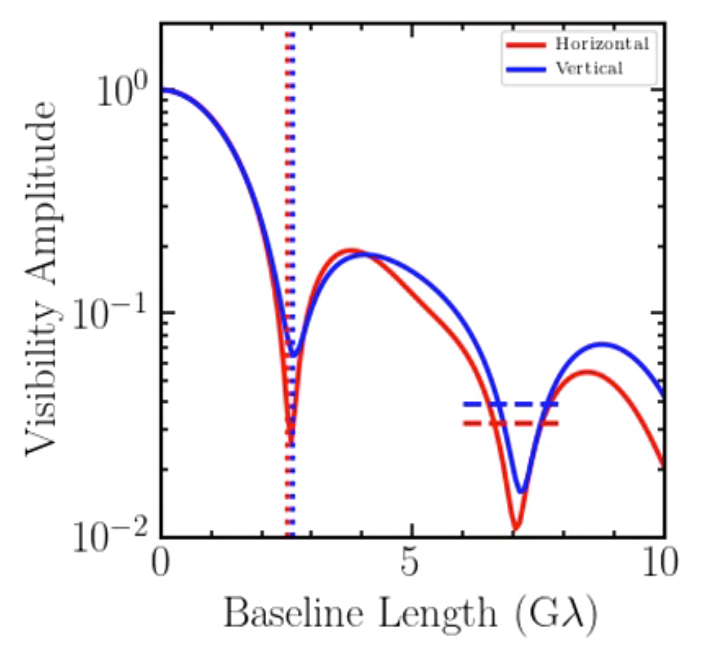
\includegraphics[width=8.5cm]{783_va}%
  %}
  %\centerline{
  %  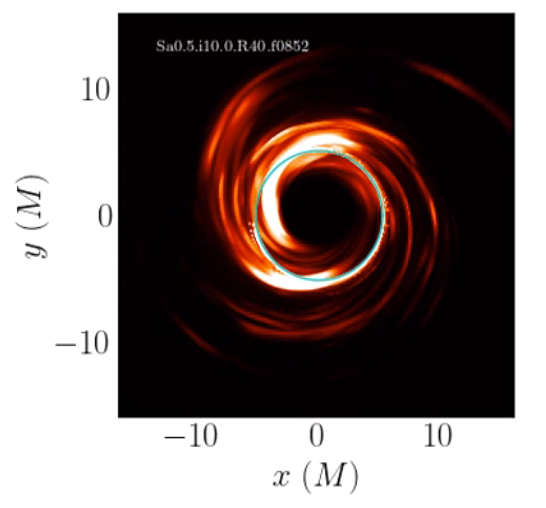
\includegraphics[width=8.5cm]{852_image}%
  %  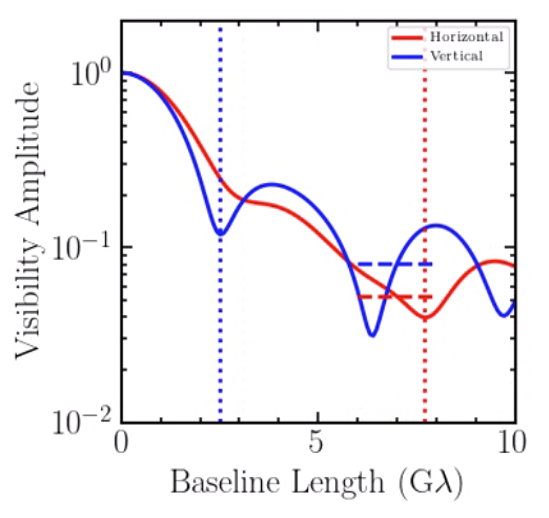
\includegraphics[width=8.5cm]{852_va}%
  %}
  [altex]
  \caption{The left panels show two snapshots from a GRMHD simulation
    with SANE field configuration and black hole spin $a=0.5$ and the
    right panels the corresponding visibility amplitudes for a
    horizontal and a vertical cross section through the images.
    The snapshot in the top row obeys both selection criteria: the
    minima are in the 2.5-3.5 G$\lambda$ range and the amplitude in
    the $6-8$G$\lambda$ is below 6\%.
    The image in the bottom row, on the other hand, is an example that
    has no minimum in one cross section and too much power at long
    baselines, due to the asymmetry introduced by a transient bright
    structure in the flow.}
  \label{fig:VA}
\end{figure*}

One way we characterize the GRMHD simulations carried out for
different black hole and flow parameters and assess their
compatibility with the \sgra\ data involves an analysis in the Fourier
domain.
To this end, we first calculate the complex visibilities by performing
a two-dimensional Fourier transform on each snapshot of each
simulation
\begin{equation}
  V(u,v) = \iint I(\alpha,\beta) e^{-2\pi i(u\alpha+v\beta)}d\alpha d\beta,
\end{equation}
where we defined $\alpha \equiv X/D$ and $\beta \equiv Y/D$, with D
being the distance to \sgra.
Figure~\ref{fig:VA} shows two example snapshots and the corresponding
visibility amplitudes (VA) as a function of baseline length for a
vertical and horizontal image cross sections from a simulation.
Even though the locations and depths of the minima in the visibility
amplitudes are primarily set by the image size, which is set by the
black hole mass, this figure shows that they can exhibit significant
variability from snapshot to snapshot because of the multitude of
structures that originate in the turbulent flow (Medeiros et
al. 2018).
In particular, the minima tend to move to larger baselines as the ring
thickness temporarily changes in response to, e.g., the appearance of
a flux tube or a similar structure.
In addition, images that have a higher degree of azimuthal asymmetry
show pronounced differences in their vertical and horizontal cross
sections.

The degree of VA variability is different from model to model and also
depends on some of the global characteristics of the flow.
For example, the overall electron density in the disk plays a role by
its effect on the ring thickness: thicker rings show more change in
the visibility minima between snapshots than thinner ones (see also
Satapathy et al. 2021 for the effect on closure phases).
Because of this, while no model is expected to resemble the observed
visibility amplitude data 100\% of the time, it is nevertheless
possible as well as discriminating to require an agreement between the
locations of the minima in each simulation snapshot and the visibility
amplitude data from \sgra\ a reasonable fraction of the time.

To carry out the comparison with the data, we focus on the VA observed
on 2017 April 7, \#3599 because that night has the best u-v coverage
near the minima.
The first visibility minima in both the N-S and E-W directions occur
between $2.5-3.5$\;G$\lambda$, as we show in
Figure~\ref{fig:data_comp}.
We define compliance for a snapshot by requiring that the VA obtained
for {\it either} the horizontal {\it or} the vertical cross section of
a snapshot have a minimum in this range of baseline lengths.

A second feature of the visibility amplitudes that can help discern
between models is the behavior of the VA at long baselines.
April 7 data also show that the amplitudes have declined to $<6\%$ of
the zero baseline flux at baselines between $6-8$\;G$\lambda$ along
all orientations.
This is characteristic of ring-like images with a relatively high
degree of azimuthal symmetry. Images that are more asymmetric, on the
other hand, lead to significantly higher amplitudes at baselines much
larger than the first minimum, or no minima at all, as the lower
panels in Figure~\ref{fig:VA} illustrate. As a result, selecting
models based on how frequently they produce snapshots with such
large-baseline power helps identify models that are in accordance with
the data.

One consideration when comparing models to data at long baselines is
the effect of interstellar scattering. Diffractive scattering has the
effect of convolving the image with a smooth kernel and can reduce the
amplitudes to $\sim 70\%$ of their intrinsic value in the
$6-8$\;G$\lambda$ range (REF).
Refractive scattering, on the other hand, introduces a noise at these
baselines of the order of $0.5-3\%$, depending on the particular
characteristics of the scattering screen toward \sgra\ (REF). To
account for both of these effects, we choose a $6\%$ upper limit to
visibility amplitudes from a model snapshot when defining compliance,
as we show in Figure~\ref{fig:data_comp}.

We assign a compliance fraction to a simulation based on the fraction
of snapshots that pass both criteria we described above. We will
discuss the results of this comparison in the next section, along with
the other model scoring criteria. [I will add to the discussion of the
  scoring table when that part is written.]

\begin{figure}
  %\centerline{ 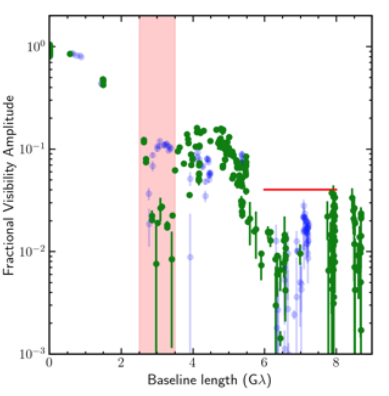
\includegraphics[width=7.5cm] {data_3599}}
  altex
  \caption{Visibility amplitude as a function of baseline length
    observed on 2017 April 7. The pink band marks the location of the
    first minima in the visibility amplitude along different
    orientations. The horizontal red line marks our conservative upper
    limit for the observed visibility amplitude between $6-8$G$\lambda$.}
\label{fig:data_comp}
\end{figure}

%==============================================================================
\subsubsection{Pre-imaging Size}

[Andrew to summarize]

%==============================================================================
\subsubsection{M-ring Diameter}

[Michi to summarize]

%==============================================================================
\subsubsection{M-ring Width}

[Michi to summarize]

%==============================================================================
\subsubsection{M-ring Asymmetry}

[Michi to summarize]

%==============================================================================
\subsection{Non-EHT Constraints}

Here we compare constraints from 86GHz, NIR, and X-ray observations.  Emission in these bands is believed to originate in the compact source from plasma that is close to or overlaps the plasma that produces the 230GHz emission observed by EHT.

It turns out that the 86GHz flux and size do not discriminate strongly between models: most models have about the right size and spectral index.  The NIR and X-ray constraints - which require that our models not overproduce the observed emission - are highly informative.  It turns out that many SANE models with large $\Rh$ (and therefore cool midplane electron populations) overproduce X-ray emission through bremsstrahlung.  In addition, many of the nonthermal models have large populations, compared to the thermal models, of electrons that are energetic enough to produce NIR emission and therefore overproduce in the NIR.   We also find that some models are dominated by Compton scattering in the NIR.

%------------------------------------------------------------------------------
\subsubsection{86 GHz Flux}

[Michi]

%------------------------------------------------------------------------------
\subsubsection{86 GHz Major Axis}

[Michi]

%------------------------------------------------------------------------------
\subsubsection{NIR Median Flux}

[Michi]

%------------------------------------------------------------------------------
\subsubsection{X-ray Luminosity}

[George to provide physical overview]

Estimates of flux from Compton.

Estimates of Bremss.  Discussion of Bremss. in SANE, large Rhigh models.

[Michi]

%==============================================================================
\subsection{Variability}

Variability is central to interpretation of Sgr A*: the small black hole size means that observations considered here are taken over intervals when the source is expected to vary significantly.  This distinguished Sgr A* from M87*, where the source is expected to vary only over timescales long compared to a single track.  

Variability is a strong constraint on the models.  Although models differ in their degree of variability, both in an integrated sense and on 4 $G\lambda$ baselines, only a very small fraction of models are as quiet as the data (these tend to be face-on SANE models).  This is true whether we use data from one day, all days, or include measurements of light curve variability from historical monitoring of Sgr A*.   In general, SANE models are quieter than MAD models, and (less strongly) face-on models are quieter than edge-on models.

If we were to apply the variability constraints directly to the models there would be M/N successful models left (M1/N for the ALMA constraint and M2/N for the visibility amplitude constraint).  One interpretation of this result is that the surviving models are the correct description of the source (although we would expect some misclassification of models as consistent or inconsistent when using 1\% cuts on such a large model set).  Another interpretation is that there is a missing physical ingredient in the models, see Section \ref{sec:discussions} for a discussion.   

\subsubsection{ALMA Light Curve}

[David Lee to provide first draft]

\subsubsection{4 $G\lambda$ Visibility Amplitude Variability}

[Boris to provide first draft]

%==============================================================================
\subsection{Best Bet Models}

[Michi to provide first draft]

We now consider combined constraints, excluding variability, under the hypothesis that (1) there is a missing physical ingredient in the models that would lower variability, but (2) that missing ingredient would not vitiate the models entirely.  Models are eliminated if they fail any one constraint.

Figure showing combined constraints for thermal models.

Figure showing combined constraints for nonthermal models.

We then inspected the remaining models and selected four best-bet models that approximately span the space of successful models.  [Written characterization of remaining models; possibly 3 or 5].  

\begin{figure*}
    \centering
    %\includegraphics{}
    [altex: a grid figure showing the $\sim$ 4 best bet models.  Each model in a column.  Top two rows are the 230GHz images and 86GHz images, last row is SEDs.]
    \caption{Best bet models.  Each column corresponds to one best bet model; top row shows a 230GHz image [average or selected image; or use GIF?]; middle row shows an 86GHz images; bottom row shows SEDs.}
    \label{fig:my_label}
\end{figure*}
